% Nama Kelompok : Android OS
% Kelas : D4 Teknik Informatika - 1A
% 1. Daffa Naufali		-
% 2. Muhammad Dzihan	- 1174095       
% 3. Nurrezky Asman		- 1174019
% 4. Yusuf Al-Qardhawi 	- 1174085

\ref{androidfigures}
\begin{figure}[ht]
\centerline{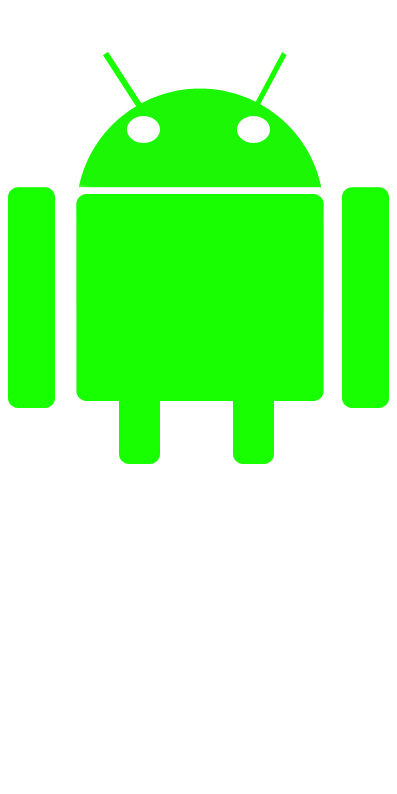
\includegraphics[width=0.25\textwidth]{figures/androidfigures.jpg}}
\caption{Ini adalag logo android}
\label{androidfigures}
\end{figure}
\section{Pengertian dan Sejarah Android}
	Android merupakan Program Operating System yang di buat dengan UNIX Based dan bawaan Sistem Kernel
	pada Bagian Hardware. Android \ref{androidfigures} pun di rilis tahun 2009 menggunakan bahasa pemrograman Java saat peluncuran pertamanya yang
	di sebarkan pada lingkungan masyarakat berdasarkan \cite{rasjid2015android}. Ketika teknologi semakin maju berkembang, Android ini memberikan dampak baik yang sangat positif
	yang menjadikan Android tersebut semakin terkenal pada semua orang sesuai platform yang semakin fleksibel untuk dipakai.
	
	\subsection{Fitur yang diluncurkan pada Android}
	Android telah menyelesaikan perkembangan dalam kurung waktu panjang ketika menghadirkan Aplikasi berguna untuk di gunakan dengan gratis berasal dari Sistem Android . Di awali
	dengan Multimedia, Games, Mode Penelitian, dan lain-lain. Fitur-Fitur tersebut memiliki kelebihan positif yang memberikan dampak pada Era Masa Depan.
	Waktu yang secara Real-Time ini membuat semakin mempercepat pengguna Android untuk saling komunikasi sesama yang lain. Karena Fitur tersebut
	membuat kita dapat melakukan Percakapan di mana saja dengan adanya koneksi internet dan Wifi untuk memudahkan sosialisasi ke masyarakat.
	Tidak hanya itu saja, Platfrom OS Android sudah dihadirkan pada pengguna ponsel atau smartphone yang memiliki fitur lebih.
	Dari Segi penampilan yang hampir sama dengan Mac OS dimana kumpulan icon tercantum di tengah bawah. Dan Tampilan yang elegan dan mudah
	dipandang keindahannnya. Berikut ini adalah fitur-fitur yang terdapat dalam android \cite{triadi2013bedah}


\section{Penggunaan Android di Mobile Phone}
Di era modern ini hampir semua orang memmpunyai Mobile Phone atau biasa kita sebut HP. \cite{triadi2013bedah}
	\ref{gambarversiandroid}
	\section{Versi-Versi Platform Android}
		Versi Android ini sendiri banyak sekali yang harus diperbaiki untuk pertama kali peluncurannya pada tahun 2009. Android ini belum memberikan sebuah nama OS Platform
		saat penyebaran berlangsung. Seiring banyak penelitian pengembangan android muncul versi-versi berikut ini: \cite{suryani2015rancang}. Versi android ini mendukung beberapa aplikasi seperti google now, google assistant, notifications, dan screen capture.
		Disetiap versinya android dilengkapi dengan API yang bertujuan untuk mengidentifikasi aplication programming interface.
\ref{gambarversiandroid}
\begin{figure}[ht]
\centerline{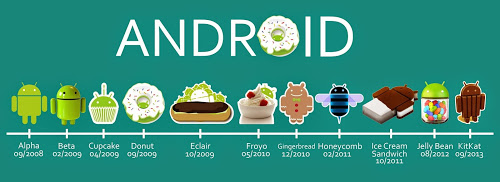
\includegraphics[width=1\textwidth]{figures/gambarversiandroid.jpg}}
\caption{Ini adalag versi android}
\label{gambarversiandroid}
\end{figure}

		\subsection{Contoh Fitur-Fitur dalam Android}
		Di dalam Android terdapat fitur-fitur penting yang wajib anda ketahui pada bagian bawaan OSnya yaitu:
		1.	Android memiliki Fitur GPS yang mencari lokasi terdekat untuk mencari keberadaan anda saat ini berdasarkan referensi \cite{anwar2014implementasi}
		2.	Android memiliki Fitur Menguatkan Sinyal saat kondisi tidak menentu.
		3.	Android memiliki Aplikasi Dukungan dari PlayStore untuk mengunduh instalasi aplikasi gratis pada smartphone
		4.	Android memiliki Daya Tahan Baterai yang cukup dan bisa bertahan dengan kondisi smartphone tidak menggunakan paket data internet
			hingga 2 hari maksimalnya.
		5.	Android memiliki aplikasi penyimpanan data yang luas untuk menyimpan data pribadi anda. Tetapi ini sangat bergantung pada spesifikasi
			Smartphone anda yang pakai saat ini. Kapasitas data saat peluncuran pertama menyediakan simpanan sekitar 1 GB, Seiring waktu berjalan
			Penyimpanan data semakin di perluas pada smartphone android hingga 32gb sampai sekarang.
		6. 	Android memiliki fitur sistem penyeimbangan hardware yang diluncurkan untuk mengoptimasikan performa smartphone untuk menghindari terjadinya
			kesalahan teknis atau istilahnya sebagai bug dalam menjalankan sistem Android. Biasanya optimasi smartphone ini dijalankan saat aplikasi digunakan
			dijalankan secara berlebihan. Contohnya bermain Mobile Legends atau Garena AOV secara tiba-tiba mengalami lag atau bug saat aplikasi berlangsung.
		7. 	Android memiliki aplikasi alarm sebagai pengganti jam dinding anda untuk membangunkan tidur anda yang terlelap. Banyak keunikan aplikasi ini,
			Anda bisa mengatur suara musik sesuai selera teman-teman semua. Selain itu bisa mengatur volume suara yang akan diujikan saat alarm berbunyi seberapa nyaringnya suara akan terdengar
		8.	Android memiliki fitur backup data yang digunakan untuk menyimpan data penting anda di server awan atau Cloud Server apabila data-data smartphonemu tidak sengaja terhapus aplikasi yang sudah diinstal sebelumnya.
			Tidak perlu khawatir tentang kehilangan data anda. Selama smartphone anda di sinkronasi secara menyeluruh, Semua data akan tersimpan dan dapat di sinkronasikan pada pengguna smartphone yang lain.
		9.	Android memiliki fitur Launcher untuk menunjukkan semua aplikasi bawaan android yang terinstal pada smartphone anda.
		10.	Android memiliki aplikasi Backup dan Restore. Berbeda dengan Cloud Server, aplikasi ini diluncurkan untuk menyimpan data anda keseluruhan pada 1 tempat tertentu baik itu cloud server ataupun lewat sd card.
			untuk disimpan sewaktu-waktu anda ingin menggantikan smartphone lama anda kepada orang lain apabila semua mau disimpan sesuai keperluan masing-masing pengguna smartphone.
		11.	Android memiliki aplikasi buku untuk dibaca pada smartphone dan dapat menggantikan buku yang berupa isi kertas dan pencetakan. Aplikasi ini sangatlah fleksibel karena bisa dibawa kemana saja tanpa perlu membawa-bawa
			buku dalam jumlah banyak. Diperlukannya sebuah SD Card untuk menyimpan buku anda di smartphone android anda.
		12.	Android memiliki aplikasi kalkulator yang menyeluruh untuk menghitung jumlah angka yang tak terhingga dengan batasan beberapa digit. Biasanya batasan digit yang dibuat oleh android sebanyak 9 angka digit
			untuk menghindari jumlah numerik tak terhingga karena kerja sistem android yang terbatas.
	\cite{anwar2014implementasi}
	\section{Kelebihan dan Kekurangan OS Android}
		OS Android ini memang bagus dari semua segala aspek, Tetapi banyak sekali yang harus kita rangkul bahwa android mempunyai dampak yang mempengaruhi penggunaan yang harus diperhatikan. Karena android pada umumnya masih banyak revisi
		yang harus diperbaiki dalam dukungan OS-Nya di seluruh smartphone untuk lebih kompatibel digunakan dan sesuai aturan pakai. Berikut Kelebihan dan Kekurangan dari OS Android.
	
	\subsection{Kelebihan OS Android}
		Inilah beberapa manfaat kelebihan pada penggunaan OS Android yaitu, sebagai berikut :
		\cite{hamka2013aplikasi}
		
	\subsection{Kekurangan OS Android}
		Mungkin anda belum sempat berpikir bahwa masih banyak kekurangan pada permasalahan yang dihadapi pada OS Android ini. Tetapi developer Android selalu mengambil langkah lebih maju untuk mengurangi
		kekurangan pada permasalahan di OS Android. Berikut beberapa kekurangan pada penggunaan OS Android.
		\cite{hamka2013aplikasi}
	
	\section{Contoh logo Android}
		Ini adalah sebuah gambar logo Android \ref{androidfigures}
		Logo ini dibuat sendiri tanpa mengambil dari Hak Cipta orang lain.
		Hak Cipta Gambar ini dibuat oleh Yusuf Al-Qardhawi dan dibuat menggunakan Adobe Photoshop Creative Cloud
		
	\section{Kesimpulan}
		Android \ref{androidfigures} memiliki banyak inovasi dalam prospek pengembangan sistem operasinya untuk menjadi lebih baik
		di masa depan. Karena tidaklah mudah membuat sesuatu yang berhasil tanpa usaha keras. Sebagai Mahasiswa
		dan Mahasiswi untuk mendukung penemu pengembangan Android ini karena tanpa mereka smartphone atau ponsel
		pada saat ini belum mengalami perubahan secara pesat.